\documentclass[conference]{IEEEtran}
\IEEEoverridecommandlockouts
% Template version as of 6/27/2024

\usepackage{cite}
\usepackage{amsmath,amssymb,amsfonts}
\usepackage{graphicx}
\usepackage{textcomp}
\usepackage{xcolor}
\usepackage{tikz}
\usepackage[caption=false,font=footnotesize]{subfig}
\definecolor{NeonRefGreen}{HTML}{39FF14}
\definecolor{RepoLinkBlue}{HTML}{0057FF}
\usepackage[colorlinks=true,linkcolor=black,citecolor=NeonRefGreen,urlcolor=RepoLinkBlue]{hyperref}
\usepackage{cleveref}
\usepackage{orcidlink}
\usepackage{eso-pic}
\usetikzlibrary{arrows.meta,calc,positioning}

\def\BibTeX{{\rm B\kern-.05em{\sc i\kern-.025em b}\kern-.08em
    T\kern-.1667em\lower.7ex\hbox{E}\kern-.125emX}}

\newif\ifanonymouspaper
\ifdefined\anonymousversion
  \anonymouspapertrue
\else
  \anonymouspaperfalse
\fi
\ifanonymouspaper
  \newcommand{\paperPdfAuthor}{Anonymous Authors}
\else
  \newcommand{\paperPdfAuthor}{Markus Baumann, Claudia Linnhoff-Popien, and Jonas Stein}
\fi

% IEEE accepted-manuscript copyright notice on page 1 (required for the arXiv posting).
\ifanonymouspaper\else
\AddToShipoutPictureFG*{%
  \AtPageLowerLeft{%
    \hspace{\dimexpr(\paperwidth-\textwidth)/2\relax}%
    \raisebox{0.35in}[0pt][0pt]{%
      \parbox[b]{\textwidth}{\scriptsize
        \copyright~2026 IEEE. Personal use of this material is permitted.
        Permission from IEEE must be obtained for all other uses, in any current
        or future media, including reprinting/republishing this material for
        advertising or promotional purposes, creating new collective works, for
        resale or redistribution to servers or lists, or reuse of any copyrighted
        component of this work in other works.}%
    }%
  }%
}
\fi
\hypersetup{
  pdftitle={Symmetry Alone Is Not an Ansatz: Task-Aligned Interactions in Equivariant Quantum Circuits},
  pdfauthor={\paperPdfAuthor},
  pdfsubject={Variational quantum learning and equivariant ansatz design},
  pdfkeywords={quantum machine learning, geometric quantum machine learning, equivariant quantum neural networks, variational quantum circuits, ansatz design, inductive bias, generalization}
}

\renewcommand{\ttdefault}{cmtt}
\renewcommand{\tableautorefname}{Tab.}
\renewcommand{\figureautorefname}{Fig.}
\renewcommand{\figurename}{Fig.}
\renewcommand{\tablename}{Tab.}
\crefname{figure}{Fig.}{Figs.}
\Crefname{figure}{Fig.}{Figs.}
\DeclareRobustCommand{\IEEEauthorrefmark}[1]{\smash{\textsuperscript{\footnotesize #1}}}

\begin{document}

\title{Symmetry Alone Is Not an Ansatz: Task-Aligned Interactions in Equivariant Quantum Circuits}

\ifanonymouspaper
\author{%
\IEEEauthorblockN{Anonymous Authors}
}
\else
\author{%
\IEEEauthorblockN{%
Markus Baumann\IEEEauthorrefmark{1}\orcidlink{0009-0007-3575-1006}\thanks{Corresponding author: \href{mailto:markus.baumann@campus.lmu.de}{markus.baumann@campus.lmu.de}.},
Claudia Linnhoff-Popien\IEEEauthorrefmark{1}\orcidlink{0000-0001-6284-9286},
and Jonas Stein\IEEEauthorrefmark{1}\orcidlink{0000-0001-5727-9151}
}
\IEEEauthorblockA{\IEEEauthorrefmark{1}\textit{QAR-Lab, Department of Computer Science, LMU Munich, Munich, Germany}}
}
\fi

\maketitle

\begin{abstract}
\input{txt/0_Abstract}
\end{abstract}

\begin{IEEEkeywords}
quantum machine learning, geometric quantum machine learning, equivariant quantum neural networks, variational quantum circuits, ansatz design, inductive bias, generalization
\end{IEEEkeywords}

\section{Introduction}
\label{sec:introduction}
\input{txt/1_Introduction}

\begin{figure*}[!t]
\centering
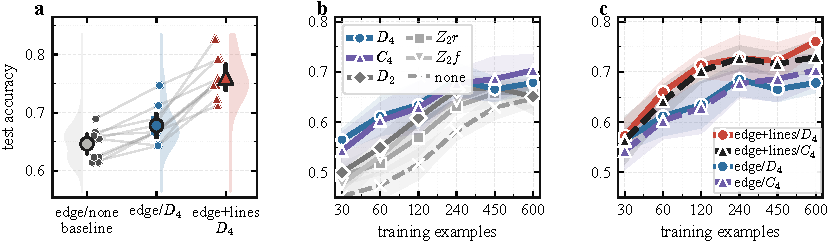
\includegraphics[width=.94\textwidth]{gfx/fig2_main_evidence}
\caption{Main empirical evidence. (a) Full $D_4$ equivariance improves the original edge ansatz over no sharing. (b) The subgroup sweep across training sizes shows that $C_4$ tracks $D_4$ closely. (c) Adding winning-line interactions to the equivariant edge ansatz improves test accuracy while preserving the imposed symmetry.}
\label{fig:main}
\end{figure*}

\section{Protocol}
\label{sec:protocol}
\input{txt/2_Protocol}

\section{Results}
\label{sec:results}
\input{txt/3_Results}

\section{Discussion}
\label{sec:discussion}
We have investigated what remains to be designed once a variational quantum learning model has been constrained to respect a data symmetry. Equivariance is a powerful inductive bias, but it is not a complete ansatz prescription. It tells the model which inputs to treat as equivalent and how to share parameters across symmetry-related parts of the data, but it leaves open how trainable capacity should be assigned to the structures of the task. Our results show that this allocation is a central part of quantum model selection.

Tic-Tac-Toe exposes this point because its symmetries and decisive winning triples are known exactly. Full $D_4$ is the natural symmetry of the board, and enforcing it improves the standard edge ansatz over an unconstrained circuit. At the same time, the subgroup sweep shows that equivariance is not all-or-nothing: in our setting, $C_4$ sharing recovers almost the same generalization behavior as full $D_4$. Thus, the strength of symmetry enforcement can itself be treated as an architectural hyperparameter. Partial symmetry can preserve most of the useful bias while avoiding some of the rigidity introduced by the full group. The choice also affects trainability: symmetry restrictions can speed up training and mitigate barren plateaus~\cite{sauvage2024building,cerezo2023simulability}, yet strongly constrained circuits may approach classically simulable regimes~\cite{cerezo2023simulability}.

The larger effect comes from the choice of interactions. The edge ansatz respects neighboring board fields, but the label is generated by complete rows, columns, and diagonals. Adding orbit-shared $ZZZ$ and $\mathrm{CCR}_Z$ gates on these winning triples keeps the model equivariant while placing trainable interactions directly on the motifs that define the task. The random-sharing, ablation, and parameter-count controls show that the improvement is not explained by fewer parameters or by adding gates indiscriminately. It comes from aligning the equivariant circuit with the geometry of the target function.

Our contribution is therefore a refinement of the symmetry program for variational quantum learning. A practical recipe is to represent the data symmetry, choose the subgroup to enforce, and place trainable interactions on label-relevant motifs. Tic-Tac-Toe is small and exactly enumerable, but precisely for this reason it exposes this principle without confounding factors. Future work should study softer versions of this recipe, such as regularized deviations or horizontal-gate constructions that interpolate between strict equivariance and fully free circuits~\cite{wiersema2025horizontal}, compare winning-line gates with parameter-matched gates on non-winning triples to isolate motif alignment, and apply motif-aligned equivariant ans\"atze to larger tasks where the relevant structures must be inferred from domain knowledge.


\section*{Appendix}
The
\ifanonymouspaper
\href{https://anonymous.4open.science/r/qc_symmetry-5FB4/}{anonymous project repository}
\else
project repository at \url{https://github.com/eybmits/vqml-symmetry}
\fi
contains the code, checked result tables, figure scripts, and manuscript
sources needed to reproduce the paper.


\ifanonymouspaper\else
\section*{Acknowledgment}
This work was supported by the LMU Sustainability Fund (EfOiE), the German
Federal Ministry of Research, Technology and Space (BMFTR) through QuCUN,
QuaRDS, and CAQAO, the Munich Quantum Valley consortia K5 and K7, and the
Bavarian Ministry of Economic Affairs project 6GQT.
\fi

\bibliographystyle{IEEEtran}
\bibliography{references}

\end{document}
